\documentclass{beamer}
%\usepackage{ngerman}
\usepackage{soul}
\usepackage{mathtools}
\usepackage{amssymb,amsmath,amsfonts}
\usepackage[utf8]{inputenc}
\usepackage{graphicx}
\usepackage{float}
\usepackage[autostyle=true,german=quotes]{csquotes}
\usepackage{gensymb}
\usepackage{units}
\usepackage{fancyhdr}
\usepackage[font=small,labelfont=bf]{caption}
\usepackage[%backend=biber,
citestyle=authortitle,
sorting=nty
]{biblatex}


\addbibresource{../../lib/lib.bib}
\addbibresource{../../solensim.bib}
\graphicspath{{../../figures/reports/}}
\graphicspath{{../../figures/}}

\setbeamertemplate{navigation symbols}{}
%\setbeamertemplate{bibliography item}{\insertbiblabel}
\setbeamertemplate{section in toc}[square]
\setbeamertemplate{subsection in toc}[square]
\setbeamertemplate{footline}[frame number]

\title{Report 06.10.20}
%\subtitle{Subtitle}
%\author{Author 1 \and Author 2}
%\date{DATE \today}

\begin{document}
%Title slide:
%\begin{frame}[plain]
%  \titlepage
%\end{frame}

%TOC slide:
%\begin{frame}
%  \frametitle{Structure}
%  \tableofcontents%[currentsection]
%\end{frame}

\begin{frame}
  \frametitle{Edge cutoff}
  \begin{figure}
    \begin{tabular}{cc}
      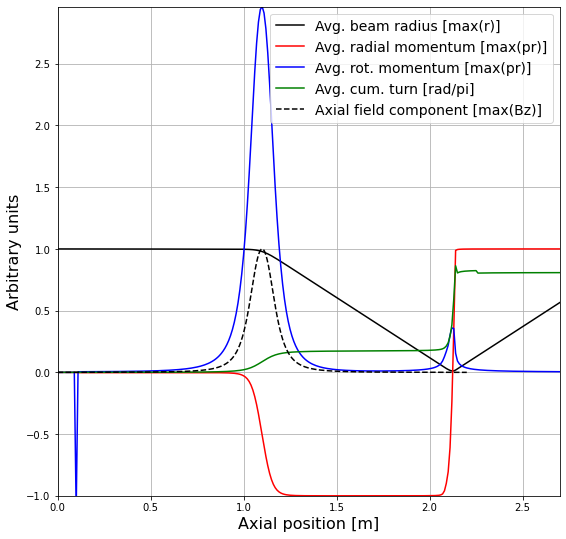
\includegraphics[width=0.5\textwidth]{uncutoff_field_durchgang} &
      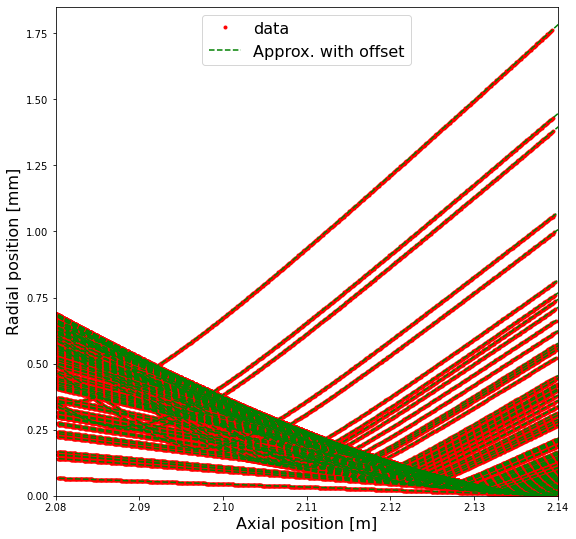
\includegraphics[width=0.5\textwidth]{uncutoff_field_focal_traj}
    \end{tabular}
  \end{figure}
  Solution:
  \[
    B_z^{cutoff} = B_z - \text{min}(B_z)
  \]
\end{frame}

\begin{frame}
  \frametitle{Scaling}
  \[
    \frac{1}{f} = \frac{e^2}{4p_z^2}\cdot F_2^N, \]
\[    k_N = \frac{B_N}{B} \propto \sqrt{\frac{F_2^N}{F_2}}, = \frac{2p_z(E_N)}{e\sqrt{f_NF_2}}
  \]
\end{frame}

\begin{frame}
  \frametitle{$\Delta f$ expansion}
  \begin{figure}
      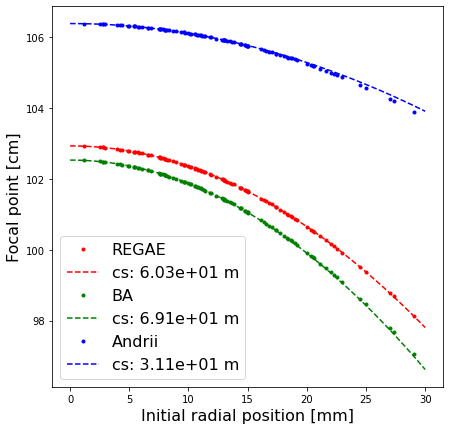
\includegraphics[width=0.6\textwidth]{cs_fit_example}
  \end{figure}
  \[ \text{Fit: } f(r) = f_0 - \Delta f(r)\]
  \[
    \Delta f = c_2\cdot r^2 + c_4\cdot r^4 + ...;\]
\[    c_s := c_2\cdot f^2\ \ \text{Approximation for small }r
  \]
\end{frame}

\begin{frame}
  \frametitle{Off-axis focusing}
  \begin{figure}
      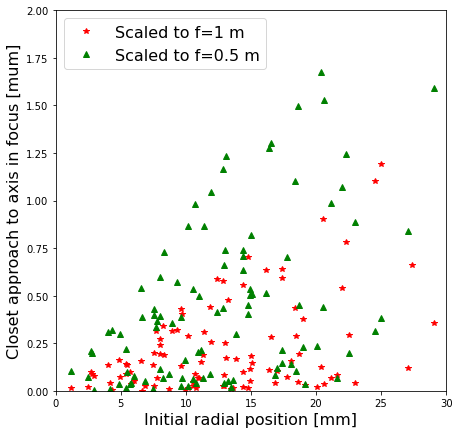
\includegraphics[width=0.6\textwidth]{weird_rmin}
  \end{figure}

\end{frame}




%\section{Section 2}
%\begin{frame}%
  %\frametitle{Title}
  %\framesubtitle{Subtitle}
%\end{frame}

%\section{Summary}
%\begin{frame}
%  \frametitle{Summary}
%  \framesubtitle{Subtitle}
%\end{frame}

%\begin{frame}[allowframebreaks]
%  \frametitle{References}
%  \printbibliography
%\end{frame}

\end{document}
